\section{Étude de faisabilité}

\subsection{Carte embarquée}

La société Jennic est un fabricant  de semi-conducteurs leader dans les solutions de connectivité sans fil. A ce titre, elle propose une gamme complète de microcontrôleurs radiofréquences faible consommation capables de gérer différents types de protocoles: IEEE802.15.4, JenNet, 6LowPAN, ZigBee PRO™\\

Le "JN5148" est probablement un des microcontrôleurs radiofréquence parmi les plus performants disponibles actuellement sur le marché. Avec sa consommation ultra basse sa très grande puissance (coeur RISC 32 Bits) et sa grande capacité mémoire (128 KB de ROM et 128 KB de RAM), ce dernier intègre un émetteur/récepteur radio 2,4 GHz tout indiqué pour la réalisation d'applications avec le protocole ZigBeePRO™ sans fil "low-cost" faible consommation.   \\

\begin{figure}[h]
\centering
\includegraphics[width=1\textwidth]{\PIXPATH/wireless}
\caption{\label{Solution Wireless Microcontroller}Schéma Fonctionnel du Microcôntroleur}
\end{figure}

\textbf{Caractéristiques}\hfill\\
%\begin{table}[h]
%\centering
\begin{longtable}{ |l|c| }
	\hline
	\multicolumn{2}{c| } {JN5148 Wireless Microcontroller}  \\
	\hline \hline
		Emetteur - Récepteur intégré \\
		 
	\hline
	Bande & 2.4 GHz compatible IEEE802.15.4\\
	\hline 
	Processeur avec cryptage & AES 128 bits\\
	\hline
	Voltage & 2.0V à 3.6V\\
	\hline
	 Mode Deep Sleep & 0.1 uA\\
	\hline
	 Mode Faible consommation avec Timer reveil & 1.1uA\\
	\hline
	 Consommation Emission & 15 A\\
	 \hline
	 Consommation Réception& 18 mA\\
	 \hline
	 Sensibilité de l'étage de réception& -95 dBm\\
	 \hline
	 Puissance de l'étage d'émission& 2.5 dBm\\
	\hline
	Caractéristiques du microcontrôleur\\
	\hline
	Processeur& RISC 32 bits (32 MIPs) mode basse consommation\\
	\hline
	ROM& 128 kB\\
	\hline
	RAM& 128 kB\\
	\hline
	Vitesse horloge& 4 de 32MHz\\
	\hline
	entrées "Analogique / Numérique"(résol. 12 bits)& 4\\
	\hline
	sorties DAC (résolution 11 bits)& 2\\
	\hline
	Comparateurs& 2\\
	\hline
	timer/compteur  & 3\\
	\hline
	entrées/sorties& Jusqu'à 21\\
	\hline
	Capteur de température& Intégré\\
	\hline
	Température de fonctionnement& -40\degres C à +85 \degres C\\
	\hline
	Boîtier & QFN 56 (8 x 8 mm)\\
	\hline
	Autres Details& Lead-free et RoHS compliant\\
	\hline
	
\end{longtable}	
%\end {table}


Le microcontrôleur "JN5148" offre une entière liberté de développement. Il sera possible de concevoir une application entièrement autonome, programmée en langage "C" dans laquelle le "JN5148" constituera le coeur du système en ayant recours à des API qui vous donneront accès aux ressources du processeur (ports d'entrées / sorties, entrées de conversion "analogique/numérique, activation des modes faible consommation, gestion des communications radio, etc...). Un environnement de développement complet avec éditeur, compilateur et débugger est à ce titre disponible en libre téléchargement.

\subsubsection{Avantages}  

\begin{enumerate}
	\item  Puce unique intégrant émetteur-récepteur et microcontrôleur pour sans fil réseaux de capteurs (permettant un coût, un encombrement et une consommation réduite de l’application).
	\item Cœpour 32 bits
	\item Consommation très faible  
	\item Capacité mémoire parmi les plus importantes du marché (pour des microcontrôleurs radiofréquence).
	\item Protocole de communication ZigBee PRO.
\end{enumerate}

\subsection{Énergie}

\subsubsection{Exigences}
\begin{itemize}

\item Autonomie: Les stations sont souvent situées dans des endroits très isolés et difficiles d'accès. Une solution est d'utiliser les ressources naturelles comme contribution à l'autonomie énergétique des stations et il est évident que la consommation électrique doit être minimale.

\smallskip \item Robustesse et Fiabilité: même en cas de problème environnemental l'approvisionnement de l'énergie à la station doit être assuré sans intervention humaine.

\smallskip \item Protection de l' environnement: les stations peuvent se trouver dans des espaces protégés donc il faut mettre en place de l'énergie non polluante et renouvelable car elle utilise des flux d'énergie naturelle(soleil, vent, eau,croissance végétale,...).
\end{itemize}

\subsubsection{Alternatives}
\begin{enumerate}
\item Énergie solaire photovolta\"ique
\begin{description}
\item [Avantages : ]
Les systèmes solaires photovoltaïques sont simples et rapides à installer, l'investissement  et le rendement sont prévisibles à long terme.
Elle répond aux exigences de robustesse et de fiabilité grâce à sa tolérance aux pannes et elle nécessite très peu de maintenance. 
Elle est exploitable pratiquement partout, la lumière du soleil étant disponible dans le monde entier. %Dans certains pays il fait nuit 6 mois l'année :p  
Aussi, cette production d'énergie ne provoque aucune perturbation pour l' environnement.

\item [Risques et inconvénients : ]
Ces installations nécessitant un apport en soleil, les pays proches des pôles, moins exposés aux rayons solaires, sont très peu rentables.
\end{description}

\item Énergie éolienne
\begin{description}
\item [Avantages : ]
L'énergie éolienne est renouvelable et est idéale car il s'agit d une forme d'énergie indéfiniment durable.
Elle ne produit pas de déchets toxiques ou radioactifs. 
Son temps de fonctionnement est d'environ 20 ans.

\item [Risques et inconvénients : ]
L'énergie éolienne varie dans le temps.  Elle tourne uniquement s'il y a du vent.
La localisation des éoliennes est dépendante de la ressource (le vent) et on ne peut pas les implanter n'importe où. 
Impact sur la faune, les études ont constaté que des éoliennes étaient responsable de la mort de quelques oiseaux.
\end{description}


\item Batterie d'accumulateurs
\begin{description}
\item [Avantages : ]
Pour une alimentation sans interruption, les batteries stockent l'énergie permettant d'alimenter de quelques minutes à quelques heures.
Il existe les batteries rechargeables qui sont orientées pour un fonctionnement avec des panneaux photovoltaïques ou  éoliennes(durée de vie augmenté, propriété anticorrosion grâces à des plaques positives épaisses, recyclable)

\item [Inconvénients : ]
Batterie à remplacer au bout d'un certain temps car ses performances
finissent par se dégrader.\\ 
Polluant.

\end{description}
\end{enumerate}

\subsubsection{Choix de solution}
Après un analyse des exigences du système nous proposons la combinaison de l'utilisation de batteries pour le stockage et pour la production une énergie renouvelable pour satisfaire l'autonomie énergétique.

\subsection{Capteurs}

    \subsubsection{Exigences}
    Les capteurs dont nous auront besoin doivent satisfaire à plusieurs
    contraintes principales: celle de la basse consommation d'énergie
    (et donc d'autonomie), celle de la précision, de la modularité (
    facilité de changement, de remplacement, de déplacement).

    \subsubsection{Solutions}
    Parmis tous les types de capteurs disponibles, ceux fonctionnant avec des
    ultrasons semblent les mieux adaptés: ils sont facilement installables donc
    évolutifs, performants et précis.

    La société française IJINUS conçoit ainsi des capteurs qui nous
    conviendraient: communicants, ils peuvent faire partie d'un
    réseau de capteurs. Ils sont en outre précis, et pas seulement
    pour des liquides en utilisant une mesure par imagerie acoustique.
    Ils sont de plus utilisables en environnement difficile, voire agressif.
    La tête de lecture est autonettoyante, permettant de ne pas avoir
    à intervenir si la tête est salle.

    Ils peuvent communiquer grâce à une interface adio optionnelle, pouvant
    être réveillés quand il y a besoin de faire une mesure. Ils transmettent
    alors la valeur de la mesure et leur niveau de charge.

    \begin{figure}[!h]
    \begin{center}
    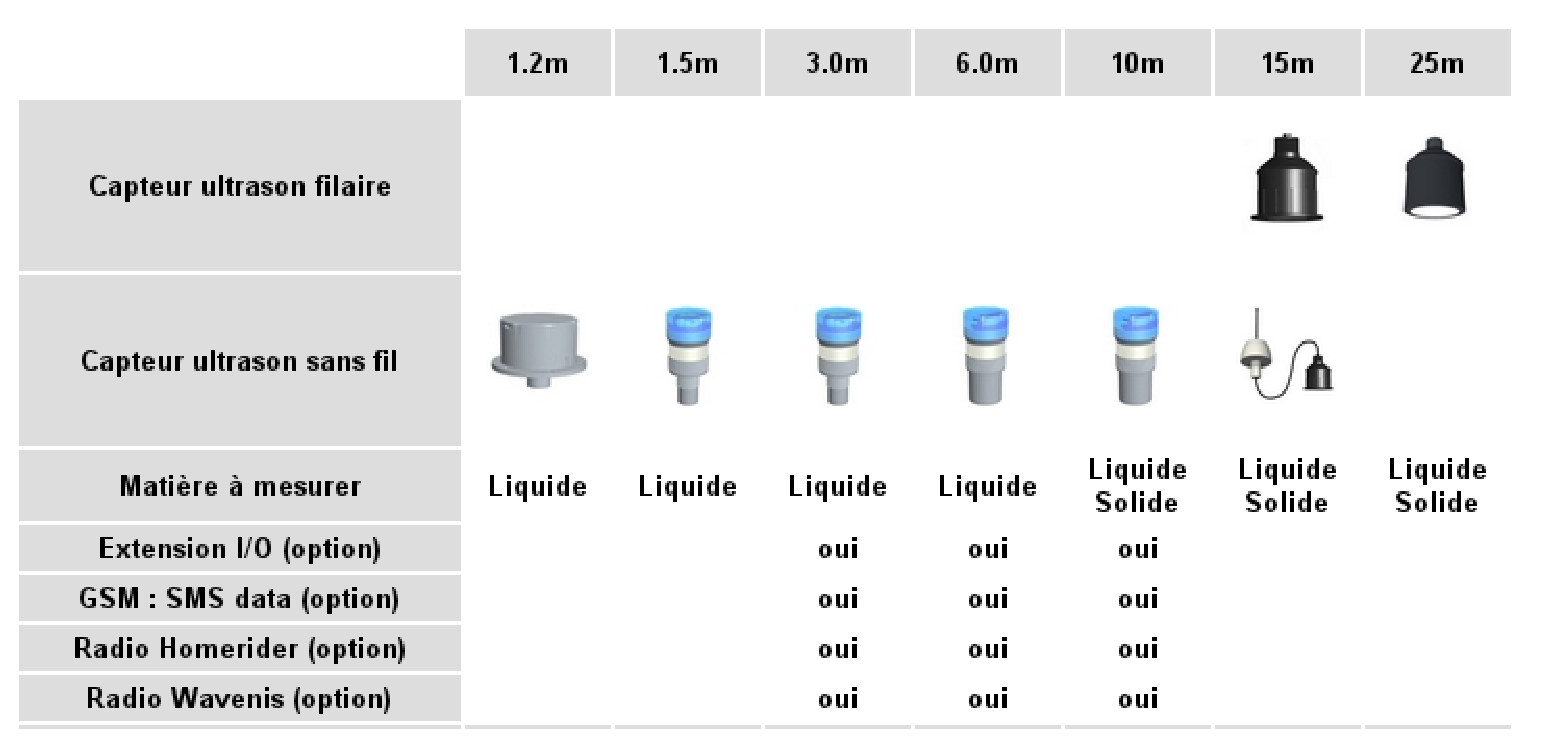
\includegraphics[width=15cm]{\PIXPATH/ijinus}
    \caption{Capteurs proposés par IJINUS}
    \end{center}
    \end{figure}

    Ce n'est pas la seule entreprise à proposer ce genre de matériel (comme la société SICK avec sa série LFVXXX), nous
    n'aurons donc a priori pas trop de mal à trouver notre bonheur au meilleur
    prix.

    \subsubsection{Conclusion}
    Le choix des capteurs demanderait une étude plus poussée
    pour trouver des capteurs correspondant précisément à nos besoins,
    ces capteurs pouvant être différents selon leur localisation.
    Les prix sont à discuter avec les fournisseurs.

\subsection{Communication}

Nous avons le choix entre plusieurs technologies différentes: la radiodiffusion, GSM/GPRS, Satelitte, 3G, WiFi, etc.

\subsubsection{Transmetteurs radio – la radiodiffusion}

La radiodiffusion a la particularité de permettre une communication asymétrique. 
Une station de radio est une installation qui émet des ondes électromagnétiques à l'aide d'un émetteur radio et d'une antenne. 
Un poste de radio ou récepteur radio est un appareil permettant de recevoir les ondes radio, en extraire la modulation et restituer les sons sur un haut-parleur.
Les transmetteurs radios ont la particularité d’être économique, par exemple, le module émetteur "NTX2-434" coûte seulement 20,51 euros. Cependant ce module a une portée de seulement 500 mètres.

    \begin{figure}[!h]
    \begin{center}
    \includegraphics[width=4cm]{\PIXPATH/moduleradio}
    \caption{}
    \end{center}
    \end{figure}

\subsubsection{GSM/GPRS}

Le protocole de transmission GSM utilise toutes les ressources disponibles pendant toute la durée de l'échange, et ne les libère qu'en fin de communication.
La norme GPRS est une dérivée du GSM qui utilise des transmissions par paquets. Cette technologie permet une communication permanente entre les sites et le système central, occupé que pendant la durée de l'échangées.
Le principal désavantage est que la couverture GPRS. Il se trouve encore inexistant sur quelques zones, comme forets, déserts.
Le module GSM/GPRS OEM "TM2" par exemple, peut être trouvé dans le marché par 45 euros. 

    \begin{figure}[!h]
    \begin{center}
    \includegraphics[width=4cm]{\PIXPATH/modulegsm}
    \caption{}
    \end{center}
    \end{figure}


\subsubsection{Satellites}

Le système de satellite peut être utilisé comme une solution complémentaire puisqu'il permet qu'on fasse la communication entre le système central et les sites qui sont situés dans les zones que le système GSM/GPRS ne couvre pas.
Le problème avec cette solution est son cout  très élevé.

\subsubsection{Choix de solution}
Après une analyse des exigences du système, nous proposons l’utilisation du module GSM/GPRS OEM "TM2". Un choix économique et que satisfait l’ensemble des exigences du projet.

\subsection{Localisation}

\subsubsection{GPS – \textsl{Global Positioning System}}

L’association d’un module GPS au système embarqué permet la localisation très précise du système. Ce module peut être totalement indépendant du reste du système, il peut communiquer directement les coordonnées au système embarqué, ou encore être associée à un système de communication indépendant qui transmettra les coordonnées relevées périodiquement au système de surveillance.
La couverture GPS est la plus complète possible, toutefois il n’est pas exclu qu’à l’occasion d’orages violents ou de perturbations électromagnétiques.

Un récepteur GPS, par exemple le GPS OEM "EM-406A", coûte environ 45 euros dans le marché. 

    \begin{figure}[!h]
    \begin{center}
    \includegraphics[width=4cm]{\PIXPATH/modulegps}
    \caption{}
    \end{center}
    \end{figure}
	
\subsubsection{Localisation par GSM/GPRS}

Basé sur le principe de la communication mobile, ce système impose de passer par un réseau satellitaire, comme le GlobalStar, qui propose des tarifs assez raisonnables. Il permet la localisation précise du système embarqué, toutefois, la couverture n’est pas assurée de partout. Certaines régions isolées peuvent subir des altérations des signaux impromptus, et d’autres encore ne sont pas du tout couvertes, telle l’Afrique Sub-Saharienne.

\subsubsection{Choix de solution}
Le système n’exige pas un module de localisation, car nos systèmes isolés sont fixés, mais pour une généricité et évolutivité du projet, nous avons ajouté cette balise. 
En premier temps, on pourrait faire le système embarqué sans ce module et quand on en aura besoin, on lui ajoute, par exemple, dans un cas d’un système mobile. 
La localisation par GPS est un peu plus chère, cependant elle nous sera plus utile, une fois que la couverture GPS est presque parfaite. On utilisera alors le module économique GPS OEM "EM-406A.
	
	
\subsection{Serveur central}

    \subsubsection{Exigences}
    Il nous faut un ensemble de serveurs capables de répondre à un grand
    nombre de requêtes, et ce en permanence. Il doit également être capable
    de conserver les traces des connexions et données reçues.

    \subsubsection{Solutions}
        \begin{enumerate}
            \item Monter nos propres serveurs
            La première solution est de monter nos propres serveurs.
            L'avantage est que nous avons les locaux pour héberger une
            telle solution, et qu'il sera possible de faire évoluer
            le parc en fonction des besoins.
    
            Les inconvénients sont cependant nombreux: il faudrait
            embaucher une équipe dédiée à la gestion de ces serveurs,
            mais également les entretenir,
            les faire évoluer. De plus, ils sont très onéreux à l'achat,
            et la consommation électrique n'est pas négligeable.
            
            \item Louer des serveurs dédiés
            Une seconde solution consiste à louer des serveurs,
            dans un \textsl{datacenter} par exemple.

            Les avantages sont nombreux: nous n'aurions pas
            à engager une équipe pour
            nous en occuper (physiquement), nous aurions une
            assurance de service
            (pouvant aller jusqu'à 99.995\% de temps en ligne)
            et nos données seraient
            en lieu sûr (les données sont souvent copiées en
            plusieurs endroits, en cas de sinistre). Là encore,
            il serait possible de trouver une offre adaptée à nos besoins.
            Nous n'aurions pas à supporter le coût du matériel et de la 
            maintenance, tout en ayant toujours un service assuré.

            Un inconvénient peut être la dépendance au service, mais ça
            n'en est pas vraiment un étant donné le nombre de
            fournisseurs sur le marché.

            Par exemple, l'entreprise OVH propose des solutions
            de serveurs dédiés très variées, pour des prix allant
            de 50 euros à plus de 600 euros par mois.

            \item Utiliser le «nuage»

            Une troisième solution consiste à héberger nos serveurs
            dans le \textsl{cloud}, nous permettant ainsi de payer
            uniquement les ressources que nous consommons, tout
            en bénéficiant d'une bonne résilience aux pannes et 
            d'une bonne disponibilité.
            L'entreprise GoGrid fournit un tel service, à partir de
            60 euros par mois. 
            

        \end{enumerate}
    \subsection{conclusion}
    Il semblerait qu'il soit préférable d'héberger les serveurs dans le \textsl{cloud}, 
    du moins pendant la phase d'exploitation. En phase de développement,
    il serait cependant possible et préférable d'avoir un petit serveur pour faire une
    mise au point à petite échelle.
%
\vfill
\pagebreak
